\subsection{Künstliche Neuronale Netze (ANN)}
\label{ann}
Können eingesetzt werden für 
\begin{itemize}
    \item überwachtes Lernen
    \item unüberwachtes Lernen
    \item Reinforcement Learning
\end{itemize}

\underline{Idee}: Komplexe Lernaufgabe wird durch viele versteckte Schichten in Teilaufgaben zerlegt. Vorteil dabei ist, dass die beim Lernalgorithmus beim Lernen der Gewichte auch selbst entscheidet, welche Zwischenkonzepte die Schichten repräsentieren $\rightarrow$ \emph{feature-engineering} (manuelle Definition der Merkmale) entfällt.\\

\emph{Feedforward}-Netzwerk: \emph{Input Layer} nimmt Eingebewerte entgegen, \emph{Output Layer} gibt Ausgabewerte aus. Dazwischen liegen \emph{Hidden Layer}, die die Eingabewerte transformieren. Ab 2 Hidden-Layern spricht man von einem \emph{Deep Neural Network}. Die einzelnen Neuronen sind in Schichten angeordnet, wobei jedes Neuron mit jedem Neuron der vorherigen Schicht \emph{gewichtet} verbunden ist.
Über die \emph{Aktivierungsfunktion} (nimmt die gewichteten Werte vorheriger Neuronen sowie einen \emph{Bias-Wert} entgegen) wird die Ausgabe eines Neurons bestimmt.
Evaluiert wird das Netzwerk über eine \emph{Verlustfunktion}, die den Fehler zwischen den Ausgaben des Netzwerks und den tatsächlichen Ausgaben berechnet.\\

\underline{\textbf{Aktivierungsfunktionen}}:\\
Die \emph{Aktivierungsfunktion} ist typischerweise in allen \emph{Hidden-Layern} gleich; im Ausgabelayer aber anwendungsabhängig und üblicherweise nicht identisch mit denen der Hidden-Layer (Regression: Ausgabe muss gesamte reellen Zahlen als Wertebereich haben; Klassifikation: Bool'sche Ausgabe (wenn binär) oder eine Wahrscheinlichkeit, ggf. auch mehrere Ausgabeneuronen für einzelne Klassen).

\begin{center}
    \begin{tabular}{c|c|c|c|c}
        \textbf{Funktion} & \textbf{Formel} & \textbf{Ableitung} & \textbf{Eigenschaften}&\textbf{Verlauf}\\
        \hline
        Threshold & \makecell{$h^{\text{thresh}}(x)=$\\$\begin{cases}1 & \text{für } x\geq 0\\0 & \text{für } x<0\end{cases}$} & nicht differenzierbar & Praxis (-)&\makecell{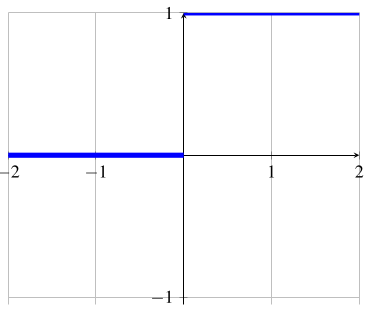
\includegraphics[width=0.15\textwidth]{deepLearning/h_tresh.png}}\\
        \hline
        Identität & $h^{\text{id}}(x)=x$ & $h^{\text{id}}(x)'=1$ & \makecell{Praxis (-);\\nur im Output bei\\Regression}&\makecell{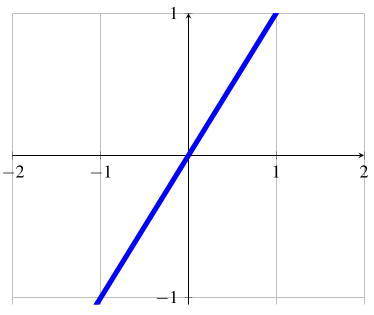
\includegraphics[width=0.15\textwidth]{deepLearning/h_id.png}}\\
        \hline
        Sigmoid & $h^{\text{logit}}(x)=\frac{1}{1+e^{-x}}$ & \makecell{$h^{\text{logit}}(x)'=$\\$h^{\text{logit}}(x)(1-h^{\text{logit}}(x))$} & \makecell{$h^{\text{logit}}(x)\in [0,1]$\\$\rightarrow$ bin. Klassifikat.} & \makecell{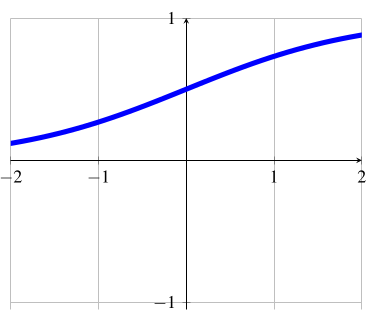
\includegraphics[width=0.15\textwidth]{deepLearning/h_logit.png}}\\
        \hline
        Hyperbol. Tangent & $h^{\text{tanh}}(x)=\frac{e^x-e^{-x}}{e^x+e^{-x}}$ & \makecell{$h^{\text{tanh}}(x)'=$\\$1-(h^{\text{tanh}}(x))^2$} & $h^{\text{tanh}}(x)\in [-1,1]$ & \makecell{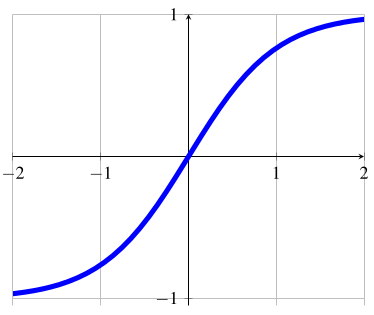
\includegraphics[width=0.15\textwidth]{deepLearning/h_tanh.png}}\\
        \hline
        \makecell{Rectified\\Linear Unit} & $h^{\text{ReLU}}(x)=\max(0,x)$ & \makecell{$h^{\text{ReLU}}(x)'=$\\$\begin{cases}0 & \text{für } x<0\\1 & \text{für } x\geq 0\end{cases}$} & $h^{\text{ReLU}}(x)\in [0,\infty)$ & \makecell{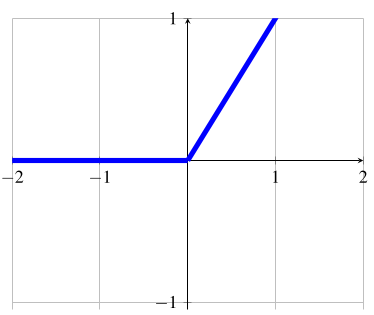
\includegraphics[width=0.15\textwidth]{deepLearning/h_relu.png}}\\
        \hline
        Softmax & & & \multicolumn{2}{c}{\makecell{$h^{\text{smax}}(x_i)\in [0,1]$\\$\sum_{i=1}^{n}h^{\text{smax}}(x_i)=1$\\$\rightarrow$ Mehrklassenklassifikation}} \\
    \end{tabular}
\end{center}

\underline{\textbf{Kosten-/Verlustfunktionen}}:\\

\begin{center}
    \begin{tabular}{c|c|c|c}
        \textbf{Funktion} & \textbf{Formel} & \textbf{Ableitung} & \textbf{Eigenschaften}\\
        \hline
        Quadratischer Fehler & \makecell{$L^{\text{qF}}(D,f)=$\\$\sum_{i=1}^{m}(f(x^{(i)})-y^{(i)})^2$} & $L'(D,f)=2(f(x)-y)$ & für $h^{\text{id}}$\\
        \hline
        Logistische Kosten & \makecell{$L^{\text{logit}}(D,f)=$\\$-\sum_{i=1}^{m}[y^{(i)}\ln(f(x^{(i)}))$\\$+(1-y^{(i)})\ln(1-f(x^{(i)}))]$} & $L'(D,f)=f(x)-y$ & \makecell{für $h^{\text{logit}}$\\ oder $h^{\text{ReLU}}$}\\
    \end{tabular}
\end{center}


Bei Verwendung der Identitätsfunktion $h^{\text{id}}=x$ als Aktivierungsfunktion und dem quadratischen Fehler $L^{\text{qF}}$ als Verlustfunktion ist die Ausgabe äquivalent zu der optimal angepassten linearen Funktion für die \underline{lineare Regression}.\\

Bei Verwendung der Sigmoid-Funktion $h^{\text{logit}}$ als Aktivierungsfunktion und der logistischen Kostenfunktion $L^{\text{logit}}$ ist die Ausgabe äquivalent zu dem optimalen Modell der \underline{logistischen Regression}.\\

\underline{\textbf{Backpropagation}}:\\
offen